% !TEX root = ../deviant.tex

\newcommand{\todofc}[1]{\todo[backgroundcolor=yellow,size=\tiny]{FC: #1}}
\newcommand{\todoinfc}[1]{\todo[inline,backgroundcolor=yellow]{FC: #1}}

\section{Experimental evaluation}
\label{sec:eval}

% Usually, an experimental evaluation of a process discovery algorithm would require to apply the proposed approach on one (or more) dataset, and to confront the learned model with those ones mined by other available approaches. However, our approach makes explicit use of information from traces labeled as ``negative'', while the totality of the approaches we could access have been designed to use positive traces only. Hence, confronting different approaches on different input data would not be fair.
% NO, questa motivazine non va bene...

One of the difficulties of evaluating process mining algorithms is that given a log, the underlying model might not be known before. As a consequence, it might be difficult to establish an \emph{ideal model} to refer and confront with. To this end, a number of metrics and evaluation indexes have been proposed in the past to evaluate how a discovered model fits a given log \todofc{Citiamo qualche metrica? O forse basta citare un paper?}. However, those metrics provide only a partial answer to the question of ``how good'' is the discovered model.\todofc{Frase molto forte, la vogliamo lasciare? Forse dovremmo almeno citare un paper che dica qualcosa di simile\ldots Notate che siccome andiamo a fare coverage del 100\%, alcune metriche ci potrebbero premiare col massimo\ldots}

A second issue is about the difficulty of confronting our approach with existing ones, especially if we consider that \todofc{Non so se questa cosa la voglio scrivere qui\ldots} our approach exploits information from traces labeled as ``negative'', while the majority of the approaches we could access have been designed to use positive traces only.

We pursued two different evaluation strategies. On one side, we defined a model, and from that model we generated a synthetic, artificial log, taking care that such log exhibit a number of desired properties: in a sense, this part of the evaluation can be referred as being about a "controlled setting". A first aim is to understand if our approach succeeds to discover a \emph{minimum} set of constraints for distinguishing positive from negative traces; a second aim is to qualitatively evaluate the discovered model, having the possibility to confront it with the original one. Experiments conducted on that synthetic log are reported and discussed in Section \ref{sec:syntheticlog}.

On the other side, we applied our discovery technique to some existing logs, thus confronting with some real data set. Again, two aims: to understand weakness and strengths of our proposal w.r.t. to some relevant literature; and to confront the proposed approach with real data (and limits and difficulties that real data bring along). Section \ref{sec:realdata} is devoted to present the selected logs and discuss the obtained results.

% Such aspect is further exacerbated by the fact that our approach exploits information from traces labeled as ``negative'', while the totality of the approaches we could access have been designed to use positive traces only.



\subsection{Experiments on a synthetic dataset}
\label{sec:syntheticlog}

% PER REFERENCE INTERBA NOSTRA:
%
% init(receive_loan_application)
% existence(assess_eligibility)
% precedence(assess_loan_risk, assess_eligibility)
% precedence(appraise_property, assess_eligibility)
% exclusive_choice(reject_application, send_acceptance_pack)
% precedence(assess_eligibility, reject_application)
% precedence(assess_eligibility, send_acceptance_pack)
% not_coexistence(reject_application, notify_approval)
% not_coexistence(receive_positive_feedback, receive_negative_feedback)
% exclusive_choice(send_acceptance_pack, receive_negative_feedback)
% precedence(appraise_property, assess_loan_risk)

% existence(0, 1, appraise_property)
% existence(0, 1, check_credit_history)
% existence(0, 1, check_income_sources)
% existence(0, 1, assess_loan_risk)
% , assess_eligibility % rimosso perché è già oggetto di un vincolo existence...
% existence(0, 1, reject_application)
% existence(0, 1, send_acceptance_pack)
% existence(0, 1, verify_receipt)
% existence(0, 1, cancel_application)
% existence(0, 1, notify_cancellation)
% existence(0, 1, approve_application)
% existence(0, 1, notify_approval)
% existence(0, 1, ask_for_customer_feedback)
% existence(0, 1, receive_positive_feedback)
% existence(0, 1, receive_negative_feedback)

The synthetic log has been generated starting from a Declare model, using the \textcolor{red}{????} tool \cite{2020-Loreti}. The model has been inspired by the Loan Application process reported in \textcolor{red}{(2018, Dumas)}. \todofc{Se abbiamo bisogno di spazio, la descrizione in NL del processo può essere saltata, e rimandiamo il lettore direttamente al disegno.} In our model, the process starts when the \emph{loan application} is received. Before \emph{assessing the eligibility}, the bank proceeds to \emph{appraise the property} of the customer, and to \emph{assess the loan risk}. Then, the bank can either \emph{reject the application} or \emph{send the acceptance pack} and, optionally, \emph{notify the approval} (if not rejected). During the process execution the bank can also \emph{receive positive} or \emph{negative feedback} (but not both), according to the experience of the loan requester. It is not expected, however, that the bank receives a \emph{negative feedback} if the \emph{acceptance pack} has been sent. Moreover, due to temporal optimization, the bank requires that the \emph{appraise of the property} is done before \emph{assessing the loan risk}.
To ease the understanding of the loan application process, a Declare model of the process is reported in Fig. \ref{fig:ex}. Moreover, all the activities have been constrained to either not be executed at all, or to be executed at most once: in Declare terminology, all the activities have been constrained to \emph{absence2}.

\begin{figure}[t]
\centering
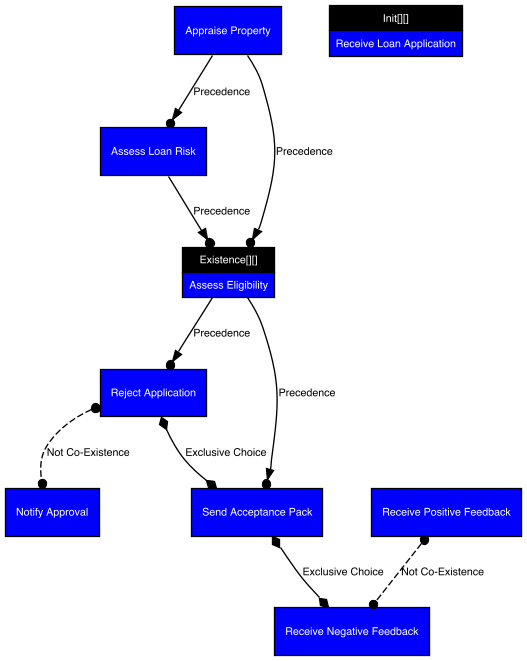
\includegraphics[width=0.6\columnwidth]{example1}
\caption{Loan approval declare process model }
\label{fig:ex}
\end{figure}

To test our approach, besides positive traces, we generated also negative traces. In particular, we generated traces that violate two different constraints:
\begin{enumerate}[label=(\alph*)]
\item the \emph{precedence(assess\_loan\_risk, assess\_eligibility)}, that is violated when either the latter activity is executed and the former is absent, or if both the activities appear in the log, but in the wrong temporal order;
%
\item the \emph{exclusive\_choice(send\_acceptance\_pack, receive\_negative\_feedback)}, that is violated when a trace either contains both the activities, or does not contain any of them.
\end{enumerate}
%
The resulting log consists of 64,000 positives traces, 25,600 traces that violates the constraint as in $(a)$, and 10,240 traces that violates the constraint as specified in $(b)$.
%
When fed with the positives traces and those traces violating an in $(a)$, our approach successfully manages to identify constraints that allow to clearly distinguish positives from negatives traces. Moreover, the discovered constraints are logically sound with the constraint that we originally decided to violate during the generation phase. When confronted with the $(b)$ scenario, our approach again successfully managed to identify a minimum model able to discriminate between positive and negative traces, and the identified constraints were indeed logically consistent with the constraint originally selected for the violation. Table \ref{tab:syntResults} summarize the obtained results and reports the first selected model for each scenario.

% source of this data:
% file:///Users/federico/Google%20Drive/on-negative-traces/experiments/2020-07-14%20Federico/run_experiments_2020-07-30_130357_CEST.html
\begin{table}
\begin{footnotesize}
\begin{tabular}{c c c c p{3cm} | p{3cm}}
\hline
Scenario & \#pos & \#neg & time & Originally violated constraint & Discovered model \\
\hline\hline
$(a)$ & 64,000 & 25,600 & 1m14.538s & \emph{precedence(assess\_loan\_ risk, assess\_eligibility)} & \emph{AlternatePrecedence( assess\_loan\_risk, assess\_eligibility)}\\
%
\hline
%
$(b)$ & 64,000 & 10,240 & 1m4.133s & \emph{exclusive\_choice( send\_acceptance\_pack, receive\_negative\_ feedback)} & \emph{ExclusiveChoice( send\_acceptance\_pack, receive\_negative\_feedback)}\\
\hline
\end{tabular}
\end{footnotesize}
\caption{Models discovered when dealing with the synthetic data set.}
\label{tab:syntResults}
\end{table}


\todoinfc{ChiaraDFM, qui ci starebbe bene un paragrafetto in cui riportiamo i risultati ottenuti usando RuM. Il commento che potremmo scrivere è che RuM trova un modello intero per coprire le positive, e riesce a distingure benissimo anche le negative: il risultato \`e atteso, dato l'elevaot numero di tracce che rende il synthetic data set molto informativo.}
% Beside positive trace, we also generated negative traces in a controlled way, i.e. taking care that those traces violate only a small, specific and known piece of the model.

% \todoinfc{x Fede, Chiara DFM, Sergio: qui bisognerebbe introdurre la metodologia per provare la validit\`a del nostro approccio, cio\`e abbiamo preso questo esempio, abbiamo generato delle tracce (cit \cite{2020-Loreti}), alcune positive, altre negative che per\`o violano dei vincoli che in questo modello non sono presenti e poi abbiamo visto se riusciamo a re-impararli. Perch\`e proprio questi vincoli e non altri?}

% A bank carries out the following \emph{loan application} process\footnote{The process is inspired by the Loan Application process reported in (2018, Dumas).} in order to grant loans. The process starts when the \emph{loan application} is received. In order to decide whether to \emph{reject the application} or to \emph{send the acceptance pack} to the customer for receiving the customer's official acceptance, the bank has to \emph{assess} the \emph{eligibility} of the loan. To this aim, the customer's \emph{property} has to be \emph{appraised} and the \emph{loan risk assessed} by the bank. The bank can optionally \emph{notify} the customer about the loan \emph{approval}, of course in case the loan is not rejected. During the process the bank can also \emph{receive positive} or \emph{negative feedback} according to the experience of the loan requester. To ease the understanding of the loan application process, a Declare model of the process is reported in Fig. \ref{fig:ex}.


% Among the processed loan application requests, some are considered as negative by the bank, while others as positive. In detail, the negative cases are the ones in which:
% \begin{itemize}
% \item the bank receives a negative feedback, although the acceptance pack is sent to the customer;
% \item the time required for carrying out the whole procedure is huge (this happens when the property appraisal is performed after the loan risk assessment).
% \end{itemize}

% Being aware of the process executions that deviate from its expectations (the negative cases), the bank would like to discover a process model of the loan application procedure in which only the positive cases are included, while the deviant ones are excluded.


\subsection{Evaluation on case studies from real data}
\label{sec:realdata}

\todoindl{x Chiara DFM: questa sezione credo sia da ripopolare da capo perch\`e l'esempio \`e cambiato}

% \subsection{Results}

